\documentclass[1p]{elsarticle_modified}
%\bibliographystyle{elsarticle-num}

%\usepackage[colorlinks]{hyperref}
%\usepackage{abbrmath_seonhwa} %\Abb, \Ascr, \Acal ,\Abf, \Afrak
\usepackage{amsfonts}
\usepackage{amssymb}
\usepackage{amsmath}
\usepackage{amsthm}
\usepackage{scalefnt}
\usepackage{amsbsy}
\usepackage{kotex}
\usepackage{caption}
\usepackage{subfig}
\usepackage{color}
\usepackage{graphicx}
\usepackage{xcolor} %% white, black, red, green, blue, cyan, magenta, yellow
\usepackage{float}
\usepackage{setspace}
\usepackage{hyperref}

\usepackage{tikz}
\usetikzlibrary{arrows}

\usepackage{multirow}
\usepackage{array} % fixed length table
\usepackage{hhline}

%%%%%%%%%%%%%%%%%%%%%
\makeatletter
\renewcommand*\env@matrix[1][\arraystretch]{%
	\edef\arraystretch{#1}%
	\hskip -\arraycolsep
	\let\@ifnextchar\new@ifnextchar
	\array{*\c@MaxMatrixCols c}}
\makeatother %https://tex.stackexchange.com/questions/14071/how-can-i-increase-the-line-spacing-in-a-matrix
%%%%%%%%%%%%%%%

\usepackage[normalem]{ulem}

\newcommand{\msout}[1]{\ifmmode\text{\sout{\ensuremath{#1}}}\else\sout{#1}\fi}
%SOURCE: \msout is \stkout macro in https://tex.stackexchange.com/questions/20609/strikeout-in-math-mode

\newcommand{\cancel}[1]{
	\ifmmode
	{\color{red}\msout{#1}}
	\else
	{\color{red}\sout{#1}}
	\fi
}

\newcommand{\add}[1]{
	{\color{blue}\uwave{#1}}
}

\newcommand{\replace}[2]{
	\ifmmode
	{\color{red}\msout{#1}}{\color{blue}\uwave{#2}}
	\else
	{\color{red}\sout{#1}}{\color{blue}\uwave{#2}}
	\fi
}

\newcommand{\Sol}{\mathcal{S}} %segment
\newcommand{\D}{D} %diagram
\newcommand{\A}{\mathcal{A}} %arc


%%%%%%%%%%%%%%%%%%%%%%%%%%%%%5 test

\def\sl{\operatorname{\textup{SL}}(2,\Cbb)}
\def\psl{\operatorname{\textup{PSL}}(2,\Cbb)}
\def\quan{\mkern 1mu \triangleright \mkern 1mu}

\theoremstyle{definition}
\newtheorem{thm}{Theorem}[section]
\newtheorem{prop}[thm]{Proposition}
\newtheorem{lem}[thm]{Lemma}
\newtheorem{ques}[thm]{Question}
\newtheorem{cor}[thm]{Corollary}
\newtheorem{defn}[thm]{Definition}
\newtheorem{exam}[thm]{Example}
\newtheorem{rmk}[thm]{Remark}
\newtheorem{alg}[thm]{Algorithm}

\newcommand{\I}{\sqrt{-1}}
\begin{document}

%\begin{frontmatter}
%
%\title{Boundary parabolic representations of knots up to 8 crossings}
%
%%% Group authors per affiliation:
%\author{Yunhi Cho} 
%\address{Department of Mathematics, University of Seoul, Seoul, Korea}
%\ead{yhcho@uos.ac.kr}
%
%
%\author{Seonhwa Kim} %\fnref{s_kim}}
%\address{Center for Geometry and Physics, Institute for Basic Science, Pohang, 37673, Korea}
%\ead{ryeona17@ibs.re.kr}
%
%\author{Hyuk Kim}
%\address{Department of Mathematical Sciences, Seoul National University, Seoul 08826, Korea}
%\ead{hyukkim@snu.ac.kr}
%
%\author{Seokbeom Yoon}
%\address{Department of Mathematical Sciences, Seoul National University, Seoul, 08826,  Korea}
%\ead{sbyoon15@snu.ac.kr}
%
%\begin{abstract}
%We find all boundary parabolic representation of knots up to 8 crossings.
%
%\end{abstract}
%\begin{keyword}
%    \MSC[2010] 57M25 
%\end{keyword}
%
%\end{frontmatter}

%\linenumbers
%\tableofcontents
%
\newcommand\colored[1]{\textcolor{white}{\rule[-0.35ex]{0.8em}{1.4ex}}\kern-0.8em\color{red} #1}%
%\newcommand\colored[1]{\textcolor{white}{ #1}\kern-2.17ex	\textcolor{white}{ #1}\kern-1.81ex	\textcolor{white}{ #1}\kern-2.15ex\color{red}#1	}

{\Large $\underline{10_{83}~(K10a_{87})}$}

\setlength{\tabcolsep}{10pt}
\renewcommand{\arraystretch}{1.6}
\vspace{1cm}\begin{tabular}{m{100pt}>{\centering\arraybackslash}m{274pt}}
\multirow{5}{120pt}{
	\centering
	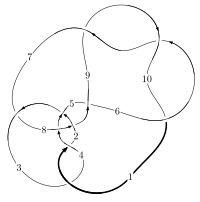
\includegraphics[width=112pt]{../../../GIT/diagram.site/Diagrams/png/167_10_83.png}\\
\ \ \ A knot diagram\footnotemark}&
\allowdisplaybreaks
\textbf{Linearized knot diagam} \\
\cline{2-2}
 &
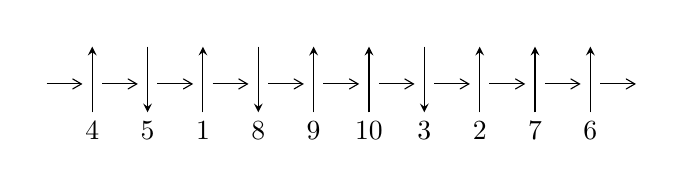
\begin{tikzpicture}[x=20pt, y=17pt]
	% nodes
	\node (C0) at (0, 0) {};
	\node (C1) at (1, 0) {};
	\node (C1U) at (1, +1) {};
	\node (C1D) at (1, -1) {4};

	\node (C2) at (2, 0) {};
	\node (C2U) at (2, +1) {};
	\node (C2D) at (2, -1) {5};

	\node (C3) at (3, 0) {};
	\node (C3U) at (3, +1) {};
	\node (C3D) at (3, -1) {1};

	\node (C4) at (4, 0) {};
	\node (C4U) at (4, +1) {};
	\node (C4D) at (4, -1) {8};

	\node (C5) at (5, 0) {};
	\node (C5U) at (5, +1) {};
	\node (C5D) at (5, -1) {9};

	\node (C6) at (6, 0) {};
	\node (C6U) at (6, +1) {};
	\node (C6D) at (6, -1) {10};

	\node (C7) at (7, 0) {};
	\node (C7U) at (7, +1) {};
	\node (C7D) at (7, -1) {3};

	\node (C8) at (8, 0) {};
	\node (C8U) at (8, +1) {};
	\node (C8D) at (8, -1) {2};

	\node (C9) at (9, 0) {};
	\node (C9U) at (9, +1) {};
	\node (C9D) at (9, -1) {7};

	\node (C10) at (10, 0) {};
	\node (C10U) at (10, +1) {};
	\node (C10D) at (10, -1) {6};
	\node (C11) at (11, 0) {};

	% arrows
	\draw[->,>={angle 60}]
	(C0) edge (C1) (C1) edge (C2) (C2) edge (C3) (C3) edge (C4) (C4) edge (C5) (C5) edge (C6) (C6) edge (C7) (C7) edge (C8) (C8) edge (C9) (C9) edge (C10) (C10) edge (C11) ;	\draw[->,>=stealth]
	(C1D) edge (C1U) (C2U) edge (C2D) (C3D) edge (C3U) (C4U) edge (C4D) (C5D) edge (C5U) (C6D) edge (C6U) (C7U) edge (C7D) (C8D) edge (C8U) (C9D) edge (C9U) (C10D) edge (C10U) ;
	\end{tikzpicture} \\
\hhline{~~} \\& 
\textbf{Solving Sequence} \\ \cline{2-2} 
 &
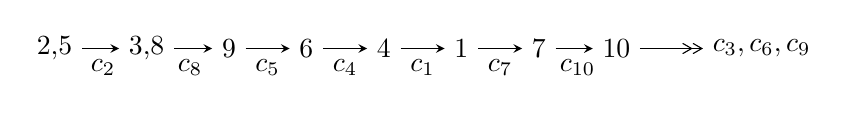
\begin{tikzpicture}[x=28pt, y=7pt]
	% node
	\node (A0) at (-1/8, 0) {2,5};
	\node (A1) at (17/16, 0) {3,8};
	\node (A2) at (17/8, 0) {9};
	\node (A3) at (25/8, 0) {6};
	\node (A4) at (33/8, 0) {4};
	\node (A5) at (41/8, 0) {1};
	\node (A6) at (49/8, 0) {7};
	\node (A7) at (57/8, 0) {10};
	\node (C1) at (1/2, -1) {$c_{2}$};
	\node (C2) at (13/8, -1) {$c_{8}$};
	\node (C3) at (21/8, -1) {$c_{5}$};
	\node (C4) at (29/8, -1) {$c_{4}$};
	\node (C5) at (37/8, -1) {$c_{1}$};
	\node (C6) at (45/8, -1) {$c_{7}$};
	\node (C7) at (53/8, -1) {$c_{10}$};
	\node (A8) at (9, 0) {$c_{3},c_{6},c_{9}$};

	% edge
	\draw[->,>=stealth]	
	(A0) edge (A1) (A1) edge (A2) (A2) edge (A3) (A3) edge (A4) (A4) edge (A5) (A5) edge (A6) (A6) edge (A7) ;
	\draw[->>,>={angle 60}]	
	(A7) edge (A8);
\end{tikzpicture} \\ 

\end{tabular} \\

\footnotetext{
The image of knot diagram is generated by the software ``\textbf{Draw programme}" developed by Andrew Bartholomew(\url{http://www.layer8.co.uk/maths/draw/index.htm\#Running-draw}), where we modified some parts for our purpose(\url{https://github.com/CATsTAILs/LinksPainter}).
}\phantom \\ \newline 
\centering \textbf{Ideals for irreducible components\footnotemark of $X_{\text{par}}$} 
 
\begin{align*}
I^u_{1}&=\langle 
5.71392\times10^{63} u^{40}+3.65753\times10^{64} u^{39}+\cdots+1.68092\times10^{63} b-3.02213\times10^{63},\\
\phantom{I^u_{1}}&\phantom{= \langle  }-6.85501\times10^{63} u^{40}-4.73991\times10^{64} u^{39}+\cdots+1.68092\times10^{63} a+1.55757\times10^{64},\;u^{41}+7 u^{40}+\cdots- u-1\rangle \\
\\
\end{align*}
\raggedright * 1 irreducible components of $\dim_{\mathbb{C}}=0$, with total 41 representations.\\
\footnotetext{All coefficients of polynomials are rational numbers. But the coefficients are sometimes approximated in decimal forms when there is not enough margin.}
\newpage
\renewcommand{\arraystretch}{1}
\centering \section*{I. $I^u_{1}= \langle 5.71\times10^{63} u^{40}+3.66\times10^{64} u^{39}+\cdots+1.68\times10^{63} b-3.02\times10^{63},\;-6.86\times10^{63} u^{40}-4.74\times10^{64} u^{39}+\cdots+1.68\times10^{63} a+1.56\times10^{64},\;u^{41}+7 u^{40}+\cdots- u-1 \rangle$}
\flushleft \textbf{(i) Arc colorings}\\
\begin{tabular}{m{7pt} m{180pt} m{7pt} m{180pt} }
\flushright $a_{2}=$&$\begin{pmatrix}1\\0\end{pmatrix}$ \\
\flushright $a_{5}=$&$\begin{pmatrix}0\\u\end{pmatrix}$ \\
\flushright $a_{3}=$&$\begin{pmatrix}1\\u^2\end{pmatrix}$ \\
\flushright $a_{8}=$&$\begin{pmatrix}4.07812 u^{40}+28.1982 u^{39}+\cdots+2.31009 u-9.26617\\-3.39928 u^{40}-21.7591 u^{39}+\cdots+7.35017 u+1.79790\end{pmatrix}$ \\
\flushright $a_{9}=$&$\begin{pmatrix}0.678844 u^{40}+6.43917 u^{39}+\cdots+9.66026 u-7.46827\\-3.39928 u^{40}-21.7591 u^{39}+\cdots+7.35017 u+1.79790\end{pmatrix}$ \\
\flushright $a_{6}=$&$\begin{pmatrix}8.89305 u^{40}+59.3831 u^{39}+\cdots-6.00010 u-11.8860\\4.09598 u^{40}+28.5050 u^{39}+\cdots+3.04934 u-8.50322\end{pmatrix}$ \\
\flushright $a_{4}=$&$\begin{pmatrix}1.80830 u^{40}+11.7114 u^{39}+\cdots-1.62251 u-0.316229\\2.98878 u^{40}+19.1668 u^{39}+\cdots-5.42693 u-3.06653\end{pmatrix}$ \\
\flushright $a_{1}=$&$\begin{pmatrix}1.80830 u^{40}+11.7114 u^{39}+\cdots-1.62251 u-0.316229\\-3.20007 u^{40}-20.2893 u^{39}+\cdots+6.28848 u+2.11978\end{pmatrix}$ \\
\flushright $a_{7}=$&$\begin{pmatrix}1.67473 u^{40}+12.2834 u^{39}+\cdots+5.93075 u-7.11966\\-3.47210 u^{40}-22.4391 u^{39}+\cdots+5.85564 u+2.70675\end{pmatrix}$ \\
\flushright $a_{10}=$&$\begin{pmatrix}-4.33853 u^{40}-24.2279 u^{39}+\cdots+19.3082 u-5.37875\\-7.53934 u^{40}-48.4715 u^{39}+\cdots+11.8342 u+6.09444\end{pmatrix}$\\&\end{tabular}
\flushleft \textbf{(ii) Obstruction class $= -1$}\\~\\
\flushleft \textbf{(iii) Cusp Shapes $= -10.0825 u^{40}-65.2708 u^{39}+\cdots+2.08186 u+7.14206$}\\~\\
\newpage\renewcommand{\arraystretch}{1}
\flushleft \textbf{(iv) u-Polynomials at the component}\newline \\
\begin{tabular}{m{50pt}|m{274pt}}
Crossings & \hspace{64pt}u-Polynomials at each crossing \\
\hline $$\begin{aligned}c_{1},c_{3}\end{aligned}$$&$\begin{aligned}
&u^{41}+u^{40}+\cdots+7 u-1
\end{aligned}$\\
\hline $$\begin{aligned}c_{2}\end{aligned}$$&$\begin{aligned}
&u^{41}-7 u^{40}+\cdots- u+1
\end{aligned}$\\
\hline $$\begin{aligned}c_{4}\end{aligned}$$&$\begin{aligned}
&u^{41}+3 u^{40}+\cdots+u+1
\end{aligned}$\\
\hline $$\begin{aligned}c_{5}\end{aligned}$$&$\begin{aligned}
&u^{41}- u^{40}+\cdots+131 u-17
\end{aligned}$\\
\hline $$\begin{aligned}c_{6},c_{9},c_{10}\end{aligned}$$&$\begin{aligned}
&u^{41}+u^{40}+\cdots+3 u-1
\end{aligned}$\\
\hline $$\begin{aligned}c_{7}\end{aligned}$$&$\begin{aligned}
&u^{41}- u^{40}+\cdots+289 u+77
\end{aligned}$\\
\hline $$\begin{aligned}c_{8}\end{aligned}$$&$\begin{aligned}
&u^{41}-3 u^{40}+\cdots-129 u+31
\end{aligned}$\\
\hline
\end{tabular}\\~\\
\newpage\renewcommand{\arraystretch}{1}
\flushleft \textbf{(v) Riley Polynomials at the component}\newline \\
\begin{tabular}{m{50pt}|m{274pt}}
Crossings & \hspace{64pt}Riley Polynomials at each crossing \\
\hline $$\begin{aligned}c_{1},c_{3}\end{aligned}$$&$\begin{aligned}
&y^{41}-29 y^{40}+\cdots-7 y-1
\end{aligned}$\\
\hline $$\begin{aligned}c_{2}\end{aligned}$$&$\begin{aligned}
&y^{41}+3 y^{40}+\cdots-7 y-1
\end{aligned}$\\
\hline $$\begin{aligned}c_{4}\end{aligned}$$&$\begin{aligned}
&y^{41}+7 y^{40}+\cdots-3 y-1
\end{aligned}$\\
\hline $$\begin{aligned}c_{5}\end{aligned}$$&$\begin{aligned}
&y^{41}-17 y^{40}+\cdots-2627 y-289
\end{aligned}$\\
\hline $$\begin{aligned}c_{6},c_{9},c_{10}\end{aligned}$$&$\begin{aligned}
&y^{41}+35 y^{40}+\cdots-3 y-1
\end{aligned}$\\
\hline $$\begin{aligned}c_{7}\end{aligned}$$&$\begin{aligned}
&y^{41}-25 y^{40}+\cdots-76331 y-5929
\end{aligned}$\\
\hline $$\begin{aligned}c_{8}\end{aligned}$$&$\begin{aligned}
&y^{41}-45 y^{40}+\cdots+24081 y-961
\end{aligned}$\\
\hline
\end{tabular}\\~\\
\newpage\flushleft \textbf{(vi) Complex Volumes and Cusp Shapes}
$$\begin{array}{c|c|c}  
\text{Solutions to }I^u_{1}& \I (\text{vol} + \sqrt{-1}CS) & \text{Cusp shape}\\
 \hline 
\begin{aligned}
u &= -0.866167 + 0.522972 I \\
a &= \phantom{-}1.35646 - 0.66908 I \\
b &= -0.725791 - 1.020460 I\end{aligned}
 & -4.89451 + 5.37316 I & \phantom{-}0.36580 - 6.73028 I \\ \hline\begin{aligned}
u &= -0.866167 - 0.522972 I \\
a &= \phantom{-}1.35646 + 0.66908 I \\
b &= -0.725791 + 1.020460 I\end{aligned}
 & -4.89451 - 5.37316 I & \phantom{-}0.36580 + 6.73028 I \\ \hline\begin{aligned}
u &= \phantom{-}0.631814 + 0.671299 I \\
a &= \phantom{-}0.943824 - 0.130258 I \\
b &= -0.620989 + 0.419528 I\end{aligned}
 & -0.99413 - 1.43665 I & -0.46376 + 2.78521 I \\ \hline\begin{aligned}
u &= \phantom{-}0.631814 - 0.671299 I \\
a &= \phantom{-}0.943824 + 0.130258 I \\
b &= -0.620989 - 0.419528 I\end{aligned}
 & -0.99413 + 1.43665 I & -0.46376 - 2.78521 I \\ \hline\begin{aligned}
u &= \phantom{-}1.134280 + 0.411388 I \\
a &= -0.871113 - 0.261658 I \\
b &= \phantom{-}0.321519 - 0.685150 I\end{aligned}
 & -6.90594 - 0.82118 I & -3.22724 + 0. I\phantom{ +0.000000I} \\ \hline\begin{aligned}
u &= \phantom{-}1.134280 - 0.411388 I \\
a &= -0.871113 + 0.261658 I \\
b &= \phantom{-}0.321519 + 0.685150 I\end{aligned}
 & -6.90594 + 0.82118 I & -3.22724 + 0. I\phantom{ +0.000000I} \\ \hline\begin{aligned}
u &= \phantom{-}0.465693 + 0.633658 I \\
a &= \phantom{-}0.05902 - 2.25820 I \\
b &= \phantom{-}0.580789 - 0.173369 I\end{aligned}
 & -0.29899 - 5.96215 I & \phantom{-}6.24062 + 8.95093 I \\ \hline\begin{aligned}
u &= \phantom{-}0.465693 - 0.633658 I \\
a &= \phantom{-}0.05902 + 2.25820 I \\
b &= \phantom{-}0.580789 + 0.173369 I\end{aligned}
 & -0.29899 + 5.96215 I & \phantom{-}6.24062 - 8.95093 I \\ \hline\begin{aligned}
u &= -0.326222 + 0.713161 I \\
a &= -2.26295 - 0.54539 I \\
b &= \phantom{-}0.755468 + 0.459159 I\end{aligned}
 & \phantom{-}2.95137 + 3.82132 I & \phantom{-}10.20968 - 8.07346 I \\ \hline\begin{aligned}
u &= -0.326222 - 0.713161 I \\
a &= -2.26295 + 0.54539 I \\
b &= \phantom{-}0.755468 - 0.459159 I\end{aligned}
 & \phantom{-}2.95137 - 3.82132 I & \phantom{-}10.20968 + 8.07346 I\\
 \hline 
 \end{array}$$\newpage$$\begin{array}{c|c|c}  
\text{Solutions to }I^u_{1}& \I (\text{vol} + \sqrt{-1}CS) & \text{Cusp shape}\\
 \hline 
\begin{aligned}
u &= -0.801624 + 1.033830 I \\
a &= -1.213990 - 0.028195 I \\
b &= \phantom{-}1.161390 + 0.790188 I\end{aligned}
 & \phantom{-}3.54673 + 5.39109 I & \phantom{-0.000000 } 0 \\ \hline\begin{aligned}
u &= -0.801624 - 1.033830 I \\
a &= -1.213990 + 0.028195 I \\
b &= \phantom{-}1.161390 - 0.790188 I\end{aligned}
 & \phantom{-}3.54673 - 5.39109 I & \phantom{-0.000000 } 0 \\ \hline\begin{aligned}
u &= \phantom{-}0.344862 + 1.265380 I \\
a &= \phantom{-}0.614486 - 0.252898 I \\
b &= -0.953366 + 0.482315 I\end{aligned}
 & -1.46534 - 1.30012 I & \phantom{-0.000000 } 0 \\ \hline\begin{aligned}
u &= \phantom{-}0.344862 - 1.265380 I \\
a &= \phantom{-}0.614486 + 0.252898 I \\
b &= -0.953366 - 0.482315 I\end{aligned}
 & -1.46534 + 1.30012 I & \phantom{-0.000000 } 0 \\ \hline\begin{aligned}
u &= \phantom{-}0.119178 + 0.652646 I \\
a &= \phantom{-}1.53296 + 2.51289 I \\
b &= -0.639883 - 0.088284 I\end{aligned}
 & \phantom{-}4.91037 - 1.30258 I & \phantom{-}16.3776 + 4.3347 I \\ \hline\begin{aligned}
u &= \phantom{-}0.119178 - 0.652646 I \\
a &= \phantom{-}1.53296 - 2.51289 I \\
b &= -0.639883 + 0.088284 I\end{aligned}
 & \phantom{-}4.91037 + 1.30258 I & \phantom{-}16.3776 - 4.3347 I \\ \hline\begin{aligned}
u &= \phantom{-}0.020565 + 0.656018 I \\
a &= \phantom{-}0.658242 - 0.704684 I \\
b &= -1.62626 - 0.29430 I\end{aligned}
 & -2.00733 - 2.04071 I & \phantom{-}3.80481 + 5.50278 I \\ \hline\begin{aligned}
u &= \phantom{-}0.020565 - 0.656018 I \\
a &= \phantom{-}0.658242 + 0.704684 I \\
b &= -1.62626 + 0.29430 I\end{aligned}
 & -2.00733 + 2.04071 I & \phantom{-}3.80481 - 5.50278 I \\ \hline\begin{aligned}
u &= -0.453284 + 0.429541 I \\
a &= \phantom{-}0.257607 - 1.211290 I \\
b &= -0.541078 - 1.041380 I\end{aligned}
 & -3.37217 + 3.66290 I & \phantom{-}0.41021 - 1.40051 I \\ \hline\begin{aligned}
u &= -0.453284 - 0.429541 I \\
a &= \phantom{-}0.257607 + 1.211290 I \\
b &= -0.541078 + 1.041380 I\end{aligned}
 & -3.37217 - 3.66290 I & \phantom{-}0.41021 + 1.40051 I\\
 \hline 
 \end{array}$$\newpage$$\begin{array}{c|c|c}  
\text{Solutions to }I^u_{1}& \I (\text{vol} + \sqrt{-1}CS) & \text{Cusp shape}\\
 \hline 
\begin{aligned}
u &= -0.439287 + 0.430084 I \\
a &= -0.369850 + 0.809872 I \\
b &= \phantom{-}0.826171 - 0.878602 I\end{aligned}
 & \phantom{-}1.92386 - 0.70569 I & \phantom{-}4.73633 - 1.49377 I \\ \hline\begin{aligned}
u &= -0.439287 - 0.430084 I \\
a &= -0.369850 - 0.809872 I \\
b &= \phantom{-}0.826171 + 0.878602 I\end{aligned}
 & \phantom{-}1.92386 + 0.70569 I & \phantom{-}4.73633 + 1.49377 I \\ \hline\begin{aligned}
u &= \phantom{-}0.458556 + 0.245803 I \\
a &= -0.926842 + 0.254373 I \\
b &= \phantom{-}3.14697 - 0.02721 I\end{aligned}
 & -1.01770 + 3.12959 I & -11.2117 + 9.6931 I \\ \hline\begin{aligned}
u &= \phantom{-}0.458556 - 0.245803 I \\
a &= -0.926842 - 0.254373 I \\
b &= \phantom{-}3.14697 + 0.02721 I\end{aligned}
 & -1.01770 - 3.12959 I & -11.2117 - 9.6931 I \\ \hline\begin{aligned}
u &= -0.98309 + 1.11338 I \\
a &= \phantom{-}1.042320 - 0.030462 I \\
b &= -1.28757 - 0.91513 I\end{aligned}
 & \phantom{-}5.88754 + 9.99849 I & \phantom{-0.000000 } 0 \\ \hline\begin{aligned}
u &= -0.98309 - 1.11338 I \\
a &= \phantom{-}1.042320 + 0.030462 I \\
b &= -1.28757 + 0.91513 I\end{aligned}
 & \phantom{-}5.88754 - 9.99849 I & \phantom{-0.000000 } 0 \\ \hline\begin{aligned}
u &= -0.164101 + 0.449464 I \\
a &= -0.688933 + 1.140020 I \\
b &= \phantom{-}0.744682 + 0.591989 I\end{aligned}
 & \phantom{-}1.35739 + 0.57043 I & \phantom{-}7.08701 - 0.51436 I \\ \hline\begin{aligned}
u &= -0.164101 - 0.449464 I \\
a &= -0.688933 - 1.140020 I \\
b &= \phantom{-}0.744682 - 0.591989 I\end{aligned}
 & \phantom{-}1.35739 - 0.57043 I & \phantom{-}7.08701 + 0.51436 I \\ \hline\begin{aligned}
u &= \phantom{-}0.95044 + 1.21876 I \\
a &= -0.641001 + 0.045558 I \\
b &= \phantom{-}0.825830 - 0.718272 I\end{aligned}
 & \phantom{-}1.17907 - 4.49890 I & \phantom{-0.000000 } 0 \\ \hline\begin{aligned}
u &= \phantom{-}0.95044 - 1.21876 I \\
a &= -0.641001 - 0.045558 I \\
b &= \phantom{-}0.825830 + 0.718272 I\end{aligned}
 & \phantom{-}1.17907 + 4.49890 I & \phantom{-0.000000 } 0\\
 \hline 
 \end{array}$$\newpage$$\begin{array}{c|c|c}  
\text{Solutions to }I^u_{1}& \I (\text{vol} + \sqrt{-1}CS) & \text{Cusp shape}\\
 \hline 
\begin{aligned}
u &= -1.11398 + 1.11513 I \\
a &= -0.963889 + 0.084455 I \\
b &= \phantom{-}1.33509 + 1.02179 I\end{aligned}
 & \phantom{-}0.7775 + 14.2581 I & \phantom{-0.000000 } 0 \\ \hline\begin{aligned}
u &= -1.11398 - 1.11513 I \\
a &= -0.963889 - 0.084455 I \\
b &= \phantom{-}1.33509 - 1.02179 I\end{aligned}
 & \phantom{-}0.7775 - 14.2581 I & \phantom{-0.000000 } 0 \\ \hline\begin{aligned}
u &= \phantom{-}0.387269\phantom{ +0.000000I} \\
a &= \phantom{-}1.11745\phantom{ +0.000000I} \\
b &= -3.36262\phantom{ +0.000000I}\end{aligned}
 & \phantom{-}3.05082\phantom{ +0.000000I} & -23.9460\phantom{ +0.000000I} \\ \hline\begin{aligned}
u &= -1.25742 + 1.12500 I \\
a &= \phantom{-}0.221918 - 0.430829 I \\
b &= -0.738517 + 0.066545 I\end{aligned}
 & \phantom{-}5.25717 - 1.92366 I & \phantom{-0.000000 } 0 \\ \hline\begin{aligned}
u &= -1.25742 - 1.12500 I \\
a &= \phantom{-}0.221918 + 0.430829 I \\
b &= -0.738517 - 0.066545 I\end{aligned}
 & \phantom{-}5.25717 + 1.92366 I & \phantom{-0.000000 } 0 \\ \hline\begin{aligned}
u &= -1.50650 + 0.79307 I \\
a &= -0.147496 + 0.451688 I \\
b &= \phantom{-}0.517015 + 0.004012 I\end{aligned}
 & \phantom{-}1.64294 + 1.58754 I & \phantom{-0.000000 } 0 \\ \hline\begin{aligned}
u &= -1.50650 - 0.79307 I \\
a &= -0.147496 - 0.451688 I \\
b &= \phantom{-}0.517015 - 0.004012 I\end{aligned}
 & \phantom{-}1.64294 - 1.58754 I & \phantom{-0.000000 } 0 \\ \hline\begin{aligned}
u &= \phantom{-}1.20335 + 1.23704 I \\
a &= \phantom{-}0.605373 + 0.022172 I \\
b &= -0.801305 + 0.846956 I\end{aligned}
 & -3.65031 - 8.13712 I & \phantom{-0.000000 } 0 \\ \hline\begin{aligned}
u &= \phantom{-}1.20335 - 1.23704 I \\
a &= \phantom{-}0.605373 - 0.022172 I \\
b &= -0.801305 - 0.846956 I\end{aligned}
 & -3.65031 + 8.13712 I & \phantom{-0.000000 } 0 \\ \hline\begin{aligned}
u &= -1.11069 + 1.42621 I \\
a &= -0.264870 + 0.387539 I \\
b &= \phantom{-}0.901140 - 0.076911 I\end{aligned}
 & \phantom{-}1.04931 - 5.53805 I & \phantom{-0.000000 } 0\\
 \hline 
 \end{array}$$\newpage$$\begin{array}{c|c|c}  
\text{Solutions to }I^u_{1}& \I (\text{vol} + \sqrt{-1}CS) & \text{Cusp shape}\\
 \hline 
\begin{aligned}
u &= -1.11069 - 1.42621 I \\
a &= -0.264870 - 0.387539 I \\
b &= \phantom{-}0.901140 + 0.076911 I\end{aligned}
 & \phantom{-}1.04931 + 5.53805 I & \phantom{-0.000000 } 0\\
 \hline 
 \end{array}$$\newpage
\newpage\renewcommand{\arraystretch}{1}
\centering \section*{ II. u-Polynomials}
\begin{tabular}{m{50pt}|m{274pt}}
Crossings & \hspace{64pt}u-Polynomials at each crossing \\
\hline $$\begin{aligned}c_{1},c_{3}\end{aligned}$$&$\begin{aligned}
&u^{41}+u^{40}+\cdots+7 u-1
\end{aligned}$\\
\hline $$\begin{aligned}c_{2}\end{aligned}$$&$\begin{aligned}
&u^{41}-7 u^{40}+\cdots- u+1
\end{aligned}$\\
\hline $$\begin{aligned}c_{4}\end{aligned}$$&$\begin{aligned}
&u^{41}+3 u^{40}+\cdots+u+1
\end{aligned}$\\
\hline $$\begin{aligned}c_{5}\end{aligned}$$&$\begin{aligned}
&u^{41}- u^{40}+\cdots+131 u-17
\end{aligned}$\\
\hline $$\begin{aligned}c_{6},c_{9},c_{10}\end{aligned}$$&$\begin{aligned}
&u^{41}+u^{40}+\cdots+3 u-1
\end{aligned}$\\
\hline $$\begin{aligned}c_{7}\end{aligned}$$&$\begin{aligned}
&u^{41}- u^{40}+\cdots+289 u+77
\end{aligned}$\\
\hline $$\begin{aligned}c_{8}\end{aligned}$$&$\begin{aligned}
&u^{41}-3 u^{40}+\cdots-129 u+31
\end{aligned}$\\
\hline
\end{tabular}\newpage\renewcommand{\arraystretch}{1}
\centering \section*{ III. Riley Polynomials}
\begin{tabular}{m{50pt}|m{274pt}}
Crossings & \hspace{64pt}Riley Polynomials at each crossing \\
\hline $$\begin{aligned}c_{1},c_{3}\end{aligned}$$&$\begin{aligned}
&y^{41}-29 y^{40}+\cdots-7 y-1
\end{aligned}$\\
\hline $$\begin{aligned}c_{2}\end{aligned}$$&$\begin{aligned}
&y^{41}+3 y^{40}+\cdots-7 y-1
\end{aligned}$\\
\hline $$\begin{aligned}c_{4}\end{aligned}$$&$\begin{aligned}
&y^{41}+7 y^{40}+\cdots-3 y-1
\end{aligned}$\\
\hline $$\begin{aligned}c_{5}\end{aligned}$$&$\begin{aligned}
&y^{41}-17 y^{40}+\cdots-2627 y-289
\end{aligned}$\\
\hline $$\begin{aligned}c_{6},c_{9},c_{10}\end{aligned}$$&$\begin{aligned}
&y^{41}+35 y^{40}+\cdots-3 y-1
\end{aligned}$\\
\hline $$\begin{aligned}c_{7}\end{aligned}$$&$\begin{aligned}
&y^{41}-25 y^{40}+\cdots-76331 y-5929
\end{aligned}$\\
\hline $$\begin{aligned}c_{8}\end{aligned}$$&$\begin{aligned}
&y^{41}-45 y^{40}+\cdots+24081 y-961
\end{aligned}$\\
\hline
\end{tabular}
\vskip 2pc
\end{document}